\documentclass{article}
\usepackage{tikz}
\usetikzlibrary{shapes.geometric, arrows, positioning}
\usepackage{geometry}
\usepackage{amsmath}

\begin{document}

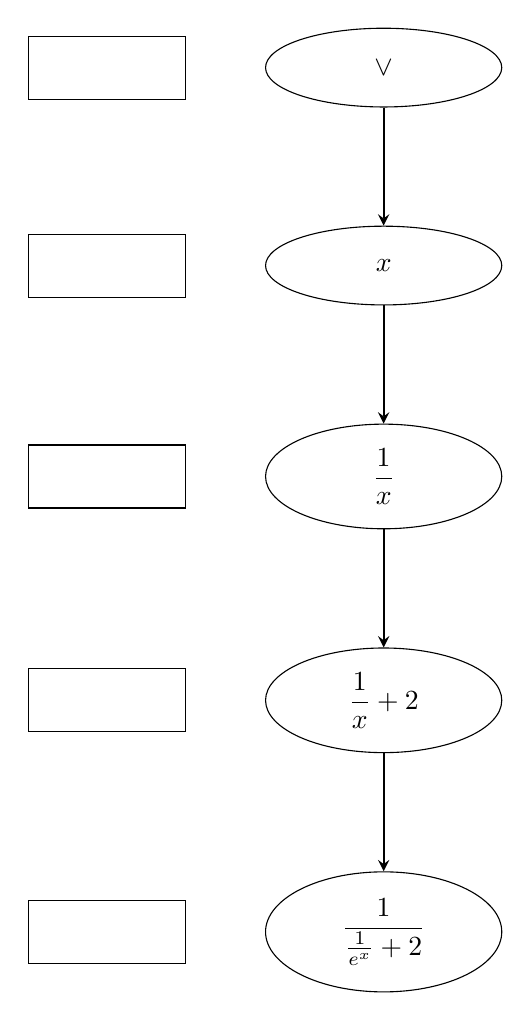
\begin{tikzpicture}[node distance=1.5cm and 1cm]

% Definir estilos para nodos
\tikzstyle{oval} = [ellipse, draw, minimum width=3cm, minimum height=1cm, align=center]
\tikzstyle{rect} = [rectangle, draw, minimum width=2cm, minimum height=0.8cm, align=center]
\tikzstyle{arrow} = [->, >=stealth, thick]

% Nodos verticales (funciones)
\node[oval] (f1) at (0,0) {$\vee$};
\node[oval] (f2) [below=of f1] {$x$};
\node[oval] (f3) [below=of f2] {$\dfrac{1}{x}$};
\node[oval] (f4) [below=of f3] {$\dfrac{1}{x} + 2$};
\node[oval] (f5) [below=of f4] {$\dfrac{1}{\frac{1}{e^x} + 2}$};

% Rectángulos a la izquierda
\node[rect, left=of f1] (l1) {};
\node[rect, left=of f2] (l2) {};
\node[rect, left=of f3] (l3) {};
\node[rect, left=of f4] (l4) {};
\node[rect, left=of f5] (l5) {};

% Flechas entre funciones
\draw[arrow] (f1) -- (f2);
\draw[arrow] (f2) -- (f3);
\draw[arrow] (f3) -- (f4);
\draw[arrow] (f4) -- (f5);

\end{tikzpicture}

\end{document}